
\documentclass[aspectratio=169,xcolor=dvipsnames]{beamer}
\usetheme{SimpleDarkBlue}

\usepackage{hyperref}
\usepackage{graphicx} % Allows including images
\usepackage{booktabs} % Allows the use of \toprule, \midrule and \bottomrule in tables
\usepackage{caption}
\usepackage{subcaption}

\usepackage{listings}



\usepackage[magyar]{babel}

%----------------------------------------------------------------------------------------
%	TITLE PAGE
%----------------------------------------------------------------------------------------

\title[short title]{Az MRC-100 műhold SZTE-s diákmoduljának szoftveres kihívásai és megoldásai} % The short title appears at the bottom of every slide, the full title is only on the title page
\subtitle{}

\author[Kiss Ádám] {Kiss Ádám}

\institute[NTU] % Your institution as it will appear on the bottom of every slide, may be shorthand to save space
{
SZTE Móra Ferenc Szakkollégium\\
SZTE Elméleti Orvostudományok Doktori Iskola\\
SZTE SZAOK Élettani Intézet -- Szenzomotoros kutatólaboratórium
     % Your institution for the title page
    \vskip 3pt
}
\date{\today} % Date, can be changed to a custom date

\begin{document}
\begin{frame}{SZTE Akadémiai modul}
\begin{columns}[c]
\column{.5\textwidth}
\begin{block}{Megvalósulás}
2022Q1-Q2, két kar, kari és intézeti költségvetésekből, a lehetőséget a BME biztosította
\end{block}
\begin{block}{Kísérletek}
	\begin{itemize}
		\item Különböző elvű hőmérséklet mérések
		\item A belső oszcillátor kalibrációs adatainak mérése
	\end{itemize}
\end{block}

\column{.45\textwidth}
	\begin{center}
		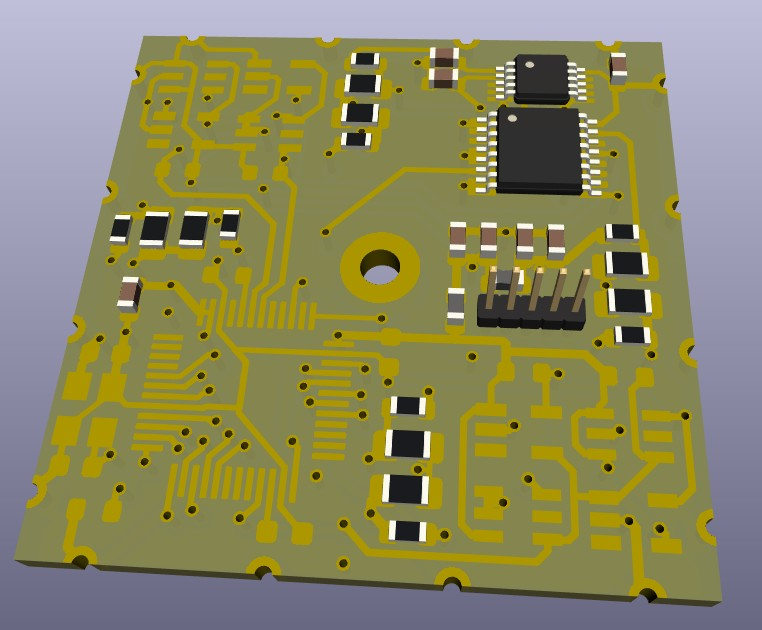
\includegraphics[width=.8\linewidth]{tanszeki3d}
	\end{center}

\end{columns}
\end{frame}

\begin{frame}{SZTE Diák-modul}
\begin{columns}
\column{.45\textwidth}
	\begin{center}
		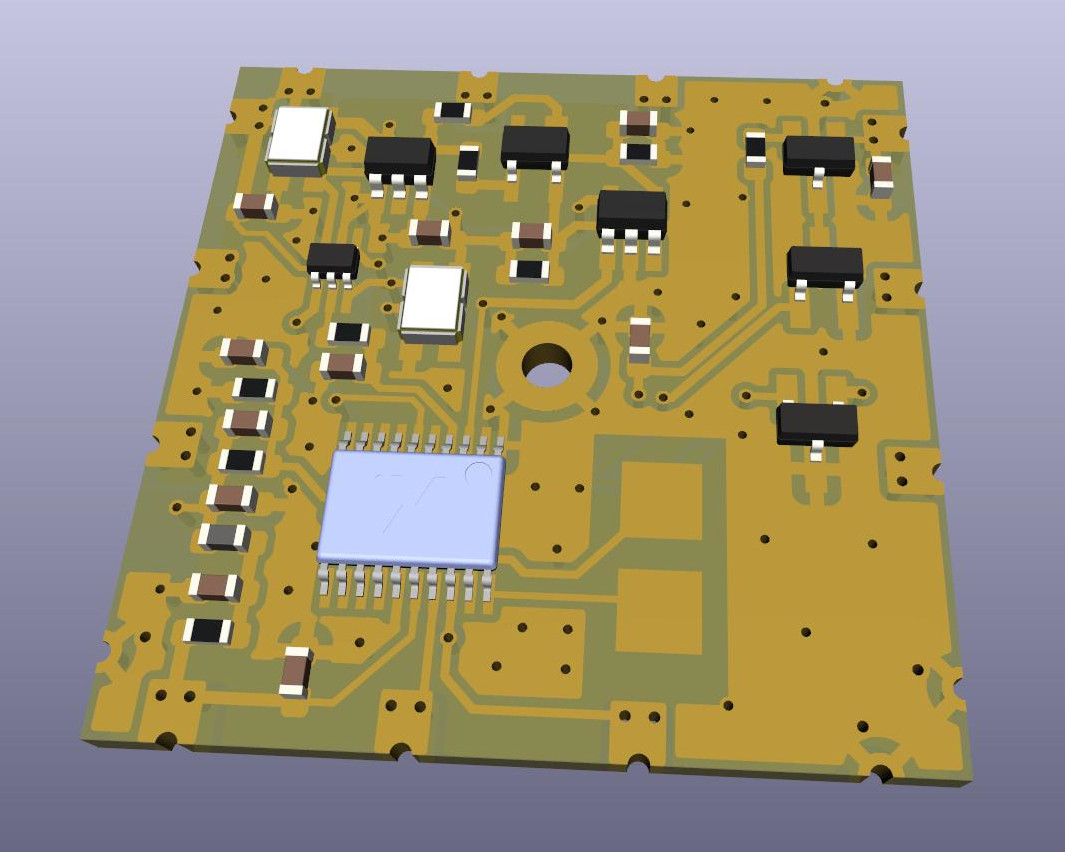
\includegraphics[width=.7\textwidth]{3d_render}
	\end{center}
	\begin{block}{Szponzoraink}
			
\includegraphics[width=0.3\linewidth]{fdh}
			
\includegraphics[width=0.17\linewidth]{ret}
			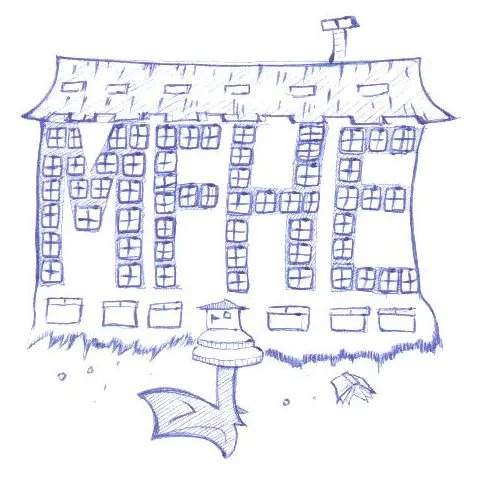
\includegraphics[width=0.17\linewidth]{mfhe}
			
\includegraphics[width=0.13\linewidth]{eurocircuits}
			
\includegraphics[width=0.15\linewidth]{csiha}
	\end{block}
\column{.5\textwidth}
	\begin{block}{Megvalósulás}
		\small{2022 szeptember 30--október 24, kizárólag diákok tervezésével és menedzselésével az SZTE Móra Ferenc Szakkollégiumban. A lehetőséget a BME biztosította.}
	\end{block}
	\begin{block}{Kísérletek}
		\begin{itemize}
			\item STM32 beépített ADC viselkedése
			\item A közös busz UART jitterének mérése modulonként
			\item Helyi bölcsész közösség idézetgyűjteménye
			\item Mágneses indukcióerősség mérés
			\item Hőmérséklet mérés
			\item TicTacToe
		\end{itemize}
	\end{block}
\end{columns}
\end{frame}

\end{document}
